\blindtext

\subsection{Smart Contracts}

Smart contracts are pieces of code that can run on the Ethereum blockchain autonomously. They can execute tasks and hold Ether or other tokens that are issued on Ethereum.

\subsection{Payment Channels}
Payment Channels are interactions between two parties that could happen on the blockchain but instead are happening off-chain. For a payment channel there are two required blockchain interactions. First, to open the channel, both parties commit a certain amount to the channel. Second, to settle the channel, a netting of the balances. The interaction in between these two steps happens off-chain with each party signing commitments and sharing them with each other. Each commitment either party signs has to trump their previous one with a higher amount. 

In figure \ref{pc_settle} the settlement case is depicted:

\begin{figure}[!t]
\centering
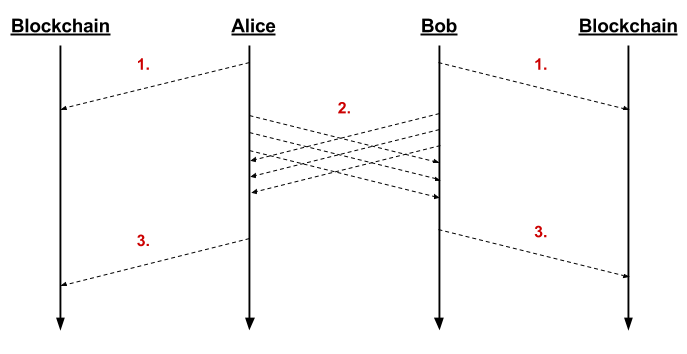
\includegraphics[width=3.0in]{images/settle.png}
\caption{The Settlement Case}
\label{pc_settle}
\end{figure}

\begin{enumerate}
\item Initial commitment and locking of funds from Alice and Bob to the payment channel.
\item Alice and Bob share transaction with each other, which can be resolved by the payment channel but instead are just collected by the participants until the channel shall be closed.
\item Alice and Bob agree on closing the channel. The channel resolves by paying the difference between the highest receipt of each party to the party with the highest receipt.
\end{enumerate}

\begin{figure}[!t]
\centering
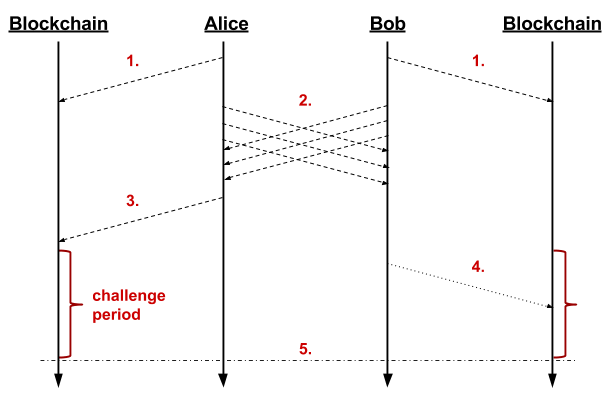
\includegraphics[width=3.0in]{images/dispute.png}
\caption{The Dispute Case}
\label{pc_dispute}
\end{figure}

In figure \ref{pc_dispute} the dispute case is depicted:

\begin{enumerate}
\item Alice and Bob lock up some tokens or a state description they control.
\item They can internally do transactions by signing receipts about new commitments and exchanging them. The receipts have to carry a nonce (sequence number) and signatures.
\item If Alice or Bob stop cooperating, the latest receipt can always be written on the blockchain. This will trigger a challenge period.
\item During this period a newer receipt (higher nonce) can be submitted.
\item After the challenge period expires, the bonded tokens are released to Alice and Bob by the ratio of the highest receipt.
\end{enumerate}

\subsection{Multi-party State Channels}


To model a round of betting as depicted in Figure \ref{mpc_round}, the internal transaction can be split into two steps:
Players submit signed receipts with betting amounts, higher amount replace lower
Sum of inputs has to be bigger/equal sum of outputs
Oracle submits signed distribution receipt, higher claim id replaces lower

\begin{figure}[!t]
\centering
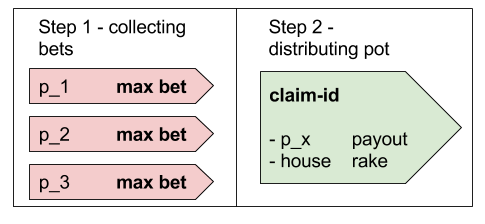
\includegraphics[width=2.5in]{images/bet.png}
\caption{Betting Round}
\label{mpc_round}
\end{figure}


\begin{figure}[!t]
\centering
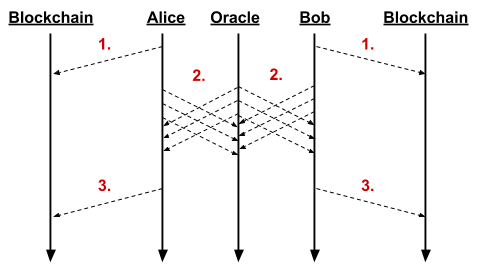
\includegraphics[width=3.0in]{images/settle2.png}
\caption{Settlement Case with Bets}
\label{mpc_settle}
\end{figure}

Figure \ref{mpc_settle} with same steps as in the payment channel:
         Lockup
         Betting rounds
         Release

